% Shared source for the student sheet and the solutions sheet.
% Content inside a solution environment appears only in the solutions PDF.

\studentonly{%
  \begin{instructions}
    Give a clear justification for each answer. You may use results proved in
    the lecture unless an exercise asks you to establish them. Questions marked
    \textbf{Extension} are optional.
  \end{instructions}}

\solutiononly{%
  \begin{instructions}
    These notes reproduce each exercise before its solution. Equivalent
    arguments, diagrams, and notation should receive full credit when the
    mathematical reasoning is correct.
  \end{instructions}}

\begin{exercise}{Translating between HMM diagrams and matrices}
  For an edge-emitting hidden Markov model, use the convention
  \[
    T^{(a)}_{ij}
      :=\Pr(X_{t+1}=a,S_{t+1}=j\mid S_t=i).
  \]
  Thus rows index the current hidden state, columns index the next hidden
  state, and the superscript records the emitted symbol. Throughout this
  exercise, $0<p,q<1$.

  \begin{parts}
    \item Suppose that $T^{(a)}_{ij}=r$. Explain each component of the
      following diagram:
      \[
        i\xrightarrow{\,a:r\,}j.
      \]
      What does a zero entry mean? Why is the matrix
      $T:=\sum_{a\in\mathcal X}T^{(a)}$ row-stochastic?

    \item \textbf{From matrices to a diagram: Zero--One--Random.}
      Take the state order to be $(0,1,R)$ and suppose that
      \[
        \eta^{(\emptyset)}
          =\begin{bmatrix}\tfrac13&\tfrac13&\tfrac13\end{bmatrix},
        \qquad
        T^{(0)}=
        \begin{bmatrix}
          0&1&0\\
          0&0&0\\
          1-p&0&0
        \end{bmatrix},
        \qquad
        T^{(1)}=
        \begin{bmatrix}
          0&0&0\\
          0&0&1\\
          p&0&0
        \end{bmatrix}.
      \]
      \begin{subparts}
        \item Draw the corresponding edge-emitting HMM. Describe informally
          the three phases represented by $0$, $1$, and $R$.

        \item Calculate $\Pr(X_{1:3}=011)$ and
          $\Pr(X_{1:3}=000)$ in two ways: first by tracing paths through your
          diagram, and then from
          \[
            \Pr(X_{1:3}=x_{1:3})
              =\eta^{(\emptyset)}
                T^{(x_1)}T^{(x_2)}T^{(x_3)}\mathbf 1.
          \]
      \end{subparts}

    \item \textbf{From a diagram to matrices: the Even Process.}
      Consider the edge-emitting HMM
      \[
        A\xrightarrow{\,0:q\,}A,
        \qquad
        A\xrightarrow{\,1:1-q\,}B,
        \qquad
        B\xrightarrow{\,1:1\,}A,
      \]
      with no other edges. Take the state order to be $(A,B)$ and let
      $\eta^{(\emptyset)}=\begin{bmatrix}\tfrac12&\tfrac12\end{bmatrix}$.
      \begin{subparts}
        \item Construct $T^{(0)}$ and $T^{(1)}$. Account explicitly for every
          zero entry in the two matrices.

        \item Form $T=T^{(0)}+T^{(1)}$ and verify that it is row-stochastic.

        \item Calculate $\Pr(X_{1:3}=011)$ and
          $\Pr(X_{1:3}=010)$ both by tracing paths through the diagram and by
          multiplying the appropriate symbol matrices. Explain how the second
          calculation reflects the defining constraint of the Even Process.
      \end{subparts}

    \item \textbf{Extension.} Let $\mathcal X$ be the observation alphabet of
      an arbitrary finite-state HMM, let
      $T=\sum_{a\in\mathcal X}T^{(a)}$, and let
      $\eta^{(\emptyset)}$ be a probability distribution. Prove that, for
      every $n\geq 0$,
      \[
        \sum_{w\in\mathcal X^n}\Pr(X_{1:n}=w)
          =\eta^{(\emptyset)}T^n\mathbf 1
          =1.
      \]
  \end{parts}

  \begin{solution}
    \begin{parts}
      \item In the diagram, $i$ is the current hidden state, $j$ is the next
        hidden state, $a$ is the emitted symbol, and $r$ is the probability of
        that joint emission-transition event conditional on starting in $i$.
        Thus the edge records
        $T^{(a)}_{ij}=\Pr(X_{t+1}=a,S_{t+1}=j\mid S_t=i)=r$.
        A zero entry means that no such emission-transition pair is possible.
        For a fixed current state $i$, the events indexed by all pairs $(a,j)$
        exhaust the possible emitted symbols and next states. Consequently,
        \[
          \sum_{a\in\mathcal X}\sum_j T^{(a)}_{ij}=1.
        \]
        Since
        \[
          T_{ij}=\sum_{a\in\mathcal X}T^{(a)}_{ij},
        \]
        every entry of $T$ is nonnegative and its $i$th row sums to
        \[
          \sum_jT_{ij}
            =\sum_j\sum_{a\in\mathcal X}T^{(a)}_{ij}=1.
        \]
        Hence $T$ is row-stochastic.

      \item
        \begin{subparts}
          \item The nonzero entries give the transitions
            \[
              0\xrightarrow{\,0:1\,}1,
              \qquad
              1\xrightarrow{\,1:1\,}R,
              \qquad
              R\xrightarrow{\,0:1-p\,}0,
              \qquad
              R\xrightarrow{\,1:p\,}0.
            \]
            Thus the diagram is a three-state cycle, with two differently
            labelled edges from $R$ to $0$. State $0$ is the phase that emits
            $0$ deterministically, state $1$ is the phase that emits $1$
            deterministically, and state $R$ is the random phase, which emits
            $1$ with probability $p$ and $0$ with probability $1-p$.

          \item For $011$, the only possible initial state is $0$. The model
            then follows
            \[
              0\xrightarrow{\,0:1\,}1
               \xrightarrow{\,1:1\,}R
               \xrightarrow{\,1:p\,}0.
            \]
            Including the initial probability $1/3$ gives
            $\Pr(011)=p/3$. Matrix multiplication gives the same result:
            \[
              \eta^{(\emptyset)}T^{(0)}T^{(1)}T^{(1)}
                =\begin{bmatrix}p/3&0&0\end{bmatrix},
              \qquad
              \Pr(011)=p/3.
            \]

            No state permits a path labelled $000$: starting from $0$, the
            first $0$ moves to state $1$, which cannot emit $0$; starting from
            $1$, even the first $0$ is impossible; and starting from $R$, the
            first two zeros move through $R\to0\to1$, after which a third zero
            is impossible. Correspondingly,
            \[
              \eta^{(\emptyset)}T^{(0)}T^{(0)}T^{(0)}
                =\begin{bmatrix}0&0&0\end{bmatrix},
              \qquad
              \Pr(000)=0.
            \]
        \end{subparts}

      \item
        \begin{subparts}
          \item In state order $(A,B)$, the matrices are
            \[
              T^{(0)}=
              \begin{bmatrix}
                q&0\\
                0&0
              \end{bmatrix},
              \qquad
              T^{(1)}=
              \begin{bmatrix}
                0&1-q\\
                1&0
              \end{bmatrix}.
            \]
            In $T^{(0)}$, the entry $(A,B)$ is zero because no $0$-edge
            connects $A$ to $B$, while the entire $B$ row is zero because
            state $B$ cannot emit $0$. In $T^{(1)}$, the diagonal entries are
            zero because neither $1$-edge is a self-loop. The two off-diagonal
            entries record $A\xrightarrow{1:1-q}B$ and
            $B\xrightarrow{1:1}A$.

          \item We have
            \[
              T=
              \begin{bmatrix}
                q&1-q\\
                1&0
              \end{bmatrix}.
            \]
            Its entries are nonnegative and both rows sum to one.

          \item The word $011$ can be produced only by starting from $A$ and
            following
            \[
              A\xrightarrow{\,0:q\,}A
               \xrightarrow{\,1:1-q\,}B
               \xrightarrow{\,1:1\,}A.
            \]
            Thus
            \[
              \Pr(011)=\frac12q(1-q).
            \]
            The matrix calculation is
            \[
              \eta^{(\emptyset)}T^{(0)}T^{(1)}T^{(1)}
                =\begin{bmatrix}\tfrac12q(1-q)&0\end{bmatrix},
              \qquad
              \Pr(011)=\frac12q(1-q).
            \]

            The word $010$ would require the path to emit a $0$ immediately
            after the transition $A\xrightarrow{1}B$, but state $B$ cannot
            emit $0$. Hence there is no such path. Equivalently,
            \[
              \eta^{(\emptyset)}T^{(0)}T^{(1)}T^{(0)}
                =\begin{bmatrix}0&0\end{bmatrix},
              \qquad
              \Pr(010)=0.
            \]
            This is the shortest example of an odd run of $1$s occurring
            between two $0$s, which the Even Process forbids.
        \end{subparts}

      \item Expanding the product of the sum of the symbol matrices gives
        \[
          T^n
            =\left(\sum_{a\in\mathcal X}T^{(a)}\right)^n
            =\sum_{w\in\mathcal X^n}T^{(w_1)}\cdots T^{(w_n)}.
        \]
        Multiplying on the left by $\eta^{(\emptyset)}$ and on the right by
        $\mathbf 1$ therefore yields
        \[
          \eta^{(\emptyset)}T^n\mathbf 1
            =\sum_{w\in\mathcal X^n}
              \eta^{(\emptyset)}T^{(w_1)}\cdots T^{(w_n)}\mathbf 1
            =\sum_{w\in\mathcal X^n}\Pr(w).
        \]
        Since $T$ is row-stochastic, $T\mathbf 1=\mathbf 1$ and hence
        $T^n\mathbf 1=\mathbf 1$. Finally,
        $\eta^{(\emptyset)}\mathbf 1=1$, because the initial vector is a
        probability distribution. The required sum is therefore one.
    \end{parts}
  \end{solution}
\end{exercise}

\newcommand{\messThreeExercise}{%
\begin{exercise}{Nonunifilar generators and large belief-state automata}
  For a belief $\eta$ and a symbol $a$ satisfying
  $\eta T^{(a)}\mathbf 1>0$, write
  \[
    F_a(\eta):=\frac{\eta T^{(a)}}{\eta T^{(a)}\mathbf 1}.
  \]
  Thus the belief-state automaton contains the transition
  \[
    \eta\xrightarrow{\,a:\eta T^{(a)}\mathbf 1\,}F_a(\eta).
  \]

  \begin{parts}
    \item \textbf{The Simple Nonunifilar Source.}
      Revisit the source from Part 2. With state order $(A,B)$, its symbol
      matrices and initial belief are
      \[
        T^{(0)}=
        \begin{bmatrix}\tfrac12&\tfrac12\\0&\tfrac12\end{bmatrix},
        \qquad
        T^{(1)}=
        \begin{bmatrix}0&0\\\tfrac12&0\end{bmatrix},
        \qquad
        \eta^{(\emptyset)}=\begin{bmatrix}\tfrac12&\tfrac12\end{bmatrix}.
      \]
      \begin{subparts}
        \item For $n\geq0$, show that
          \[
            \eta^{(10^n)}=
              \begin{bmatrix}\dfrac1{n+1}&\dfrac n{n+1}\end{bmatrix},
            \qquad
            \eta^{(0^n)}=
              \begin{bmatrix}\dfrac1{n+2}&\dfrac{n+1}{n+2}\end{bmatrix}.
          \]
          Deduce that
          $\eta^{(0^n)}=\eta^{(10^{n+1})}$ and observe that
          $\eta^{(\emptyset)}=\eta^{(10)}$.

        \item Show that, for every $n\geq1$,
          \[
            \eta^{(10^n1)}=\eta^{(1)}.
          \]

        \item Draw the first four states of the belief-state automaton and
          indicate its continuing structure with an ellipsis. Show that the
          beliefs $\eta^{(10^n)}$ are all distinct, identify their limiting
          point in the $1$-simplex, and explain why the two-state generator
          produces a countably infinite belief-state automaton.
      \end{subparts}

    \item \textbf{Mess3.}
      Now take hidden-state and symbol sets both equal to $\{0,1,2\}$, with
      \[
        \alpha=\frac15,\qquad b=\frac{1-\alpha}{2}=\frac25,
        \qquad x=\frac3{20},\qquad y=1-2x=\frac7{10},
      \]
      and
      \[
        \begin{aligned}
          T^{(0)}&=
          \begin{bmatrix}
            \alpha y&bx&bx\\ \alpha x&by&bx\\ \alpha x&bx&by
          \end{bmatrix},&
          T^{(1)}&=
          \begin{bmatrix}
            by&\alpha x&bx\\ bx&\alpha y&bx\\ bx&\alpha x&by
          \end{bmatrix},\\[1mm]
          T^{(2)}&=
          \begin{bmatrix}
            by&bx&\alpha x\\ bx&by&\alpha x\\ bx&bx&\alpha y
          \end{bmatrix},&
          \eta^{(\emptyset)}&=
          \begin{bmatrix}\tfrac13&\tfrac13&\tfrac13\end{bmatrix}.
        \end{aligned}
      \]
      \begin{subparts}
        \item Verify that $T=\sum_{a=0}^2T^{(a)}$ is row-stochastic and
          explain why this generator is nonunifilar. Compute
          $\eta^{(0)},\eta^{(1)}$, and $\eta^{(2)}$.

        \item Compute $\eta^{(00)},\eta^{(01)}$, and $\eta^{(02)}$. Use the
          cyclic symmetry of the process to sketch the first two generations
          of the belief-state automaton, including the symbol labels.

        \item Compute the next-token matrix $A$, with
          $A_{ia}=\sum_jT^{(a)}_{ij}$, and show that it is invertible. What
          does this imply about whether distinct beliefs can be merged by the
          map $p^{(x_{1:n})}=\eta^{(x_{1:n})}A$? Contrast this with Exercise 2.

        \item Using a short program, form
          \[
            \mathcal B_d:=
            \bigl\{\eta^{(x_{1:d})}:x_{1:d}\in\{0,1,2\}^d\bigr\},
            \qquad 0\leq d\leq7.
          \]
          Record the number of distinct beliefs at each depth. Visualise
          $\mathcal B_7$ on the hidden-state $2$-simplex, colouring each point
          by its final symbol. Also visualise the associated next-token
          vectors on the symbol $2$-simplex. Describe the geometric structure
          that emerges and how the three maps $F_0,F_1,F_2$ generate the
          outgoing transitions of the belief-state automaton.

        \item Explain why the belief-state automata constructed in this
          exercise are unifilar even though their generators are not. Compare
          the ladder-with-resets structure of the Simple Nonunifilar Source
          with the branching structure of Mess3. Finally, explain why the set
          of beliefs reached by finite histories is countable even though its
          closure can have a much richer fractal geometry.
      \end{subparts}
  \end{parts}

  \begin{solution}
    \begin{parts}
      \item
        \begin{subparts}
          \item After observing $1$, the hidden state is $A$. A path emitting
            the following $0^n$ either remains in $A$ throughout or moves from
            $A$ to $B$ after one of the $n$ emissions. These $n+1$ paths have
            equal weight $2^{-n}$; one ends in $A$ and $n$ end in $B$. Thus
            \[
              \eta^{(1)}(T^{(0)})^n
                =2^{-n}\begin{bmatrix}1&n\end{bmatrix},
              \qquad
              \eta^{(10^n)}=
                \begin{bmatrix}\dfrac1{n+1}&\dfrac n{n+1}\end{bmatrix}.
            \]
            Starting instead from the uniform initial belief gives
            \[
              \eta^{(\emptyset)}(T^{(0)})^n
                =2^{-(n+1)}\begin{bmatrix}1&n+1\end{bmatrix},
              \qquad
              \eta^{(0^n)}=
                \begin{bmatrix}\dfrac1{n+2}&\dfrac{n+1}{n+2}\end{bmatrix}.
            \]
            Hence $\eta^{(0^n)}=\eta^{(10^{n+1})}$, and the case $n=0$
            gives $\eta^{(\emptyset)}=\eta^{(10)}$.

          \item For $n\geq1$, direct multiplication gives
            \[
              \eta^{(10^n)}T^{(1)}
                =\begin{bmatrix}\dfrac n{2(n+1)}&0\end{bmatrix}.
            \]
            Normalising yields
            $\eta^{(10^n1)}=\begin{bmatrix}1&0\end{bmatrix}=\eta^{(1)}$.

          \item The automaton begins
            \[
              \eta^{(1)}\xrightarrow{\,0\,}\eta^{(10)}
              \xrightarrow{\,0\,}\eta^{(100)}
              \xrightarrow{\,0\,}\eta^{(1000)}
              \xrightarrow{\,0\,}\cdots,
            \]
            and every $\eta^{(10^n)}$ with $n\geq1$ has a $1$-transition
            back to $\eta^{(1)}$. Since the first coordinate
            $1/(n+1)$ is different for each $n$, the beliefs are distinct, and
            \[
              \lim_{n\to\infty}\eta^{(10^n)}
                =\begin{bmatrix}0&1\end{bmatrix}.
            \]
            This limiting belief is not reached after any finite history.
            Hence the two hidden generator states induce countably infinitely
            many reachable beliefs.
        \end{subparts}

      \item
        \begin{subparts}
          \item Substitution gives
            $\alpha y=7/50$, $bx=3/50$, $\alpha x=3/100$, and
            $by=7/25$. Each entry is positive, and every state has several
            possible destinations for each emitted symbol, so the generator
            is nonunifilar. The rows of $T^{(0)}+T^{(1)}+T^{(2)}$ each sum to
            one. By multiplying the uniform belief and normalising,
            \[
              \eta^{(0)}=\begin{bmatrix}\tfrac15&\tfrac25&\tfrac25\end{bmatrix},
              \quad
              \eta^{(1)}=\begin{bmatrix}\tfrac25&\tfrac15&\tfrac25\end{bmatrix},
              \quad
              \eta^{(2)}=\begin{bmatrix}\tfrac25&\tfrac25&\tfrac15\end{bmatrix}.
            \]

          \item Updating $\eta^{(0)}$ by each symbol gives
            \[
              \eta^{(00)}=
                \begin{bmatrix}\tfrac{13}{87}&\tfrac{37}{87}&\tfrac{37}{87}\end{bmatrix},
              \quad
              \eta^{(01)}=
                \begin{bmatrix}\tfrac{52}{163}&\tfrac{37}{163}&\tfrac{74}{163}\end{bmatrix},
              \quad
              \eta^{(02)}=
                \begin{bmatrix}\tfrac{52}{163}&\tfrac{74}{163}&\tfrac{37}{163}\end{bmatrix}.
            \]
            Cyclically permuting both the state coordinates and symbol labels
            gives the remaining six depth-two beliefs. The root has three
            symbol-labelled children, and each of those children again has
            three symbol-labelled successors.

          \item Summing over destination states gives
            \[
              A=\begin{bmatrix}
                \tfrac{13}{50}&\tfrac{37}{100}&\tfrac{37}{100}\\
                \tfrac{37}{100}&\tfrac{13}{50}&\tfrac{37}{100}\\
                \tfrac{37}{100}&\tfrac{37}{100}&\tfrac{13}{50}
              \end{bmatrix}.
            \]
            Its eigenvalues are $1,-11/100,-11/100$, so
            $\det A=121/10000\neq0$. Consequently
            $\eta A=\eta' A$ implies $\eta=\eta'$: the next-token readout
            does not merge distinct Mess3 beliefs. In Exercise 2 the
            corresponding matrix has a nontrivial kernel and maps
            $\eta^{(01)}$ and $\eta^{(10)}$ to the same next-token vector.

          \item For these parameters, numerical enumeration gives
            \[
              \begin{array}{c|rrrrrrrr}
                d&0&1&2&3&4&5&6&7\\ \hline
                |\mathcal B_d|&1&3&9&27&81&243&729&2187
              \end{array}
            \]
            with no coincidences at the displayed depths. The plots show
            three recursively repeated clusters forming a fractal pattern.
            The next-token plot is an invertible linear image of the belief
            plot, so it preserves the distinct points and their recursive
            organisation.

            \begin{center}
              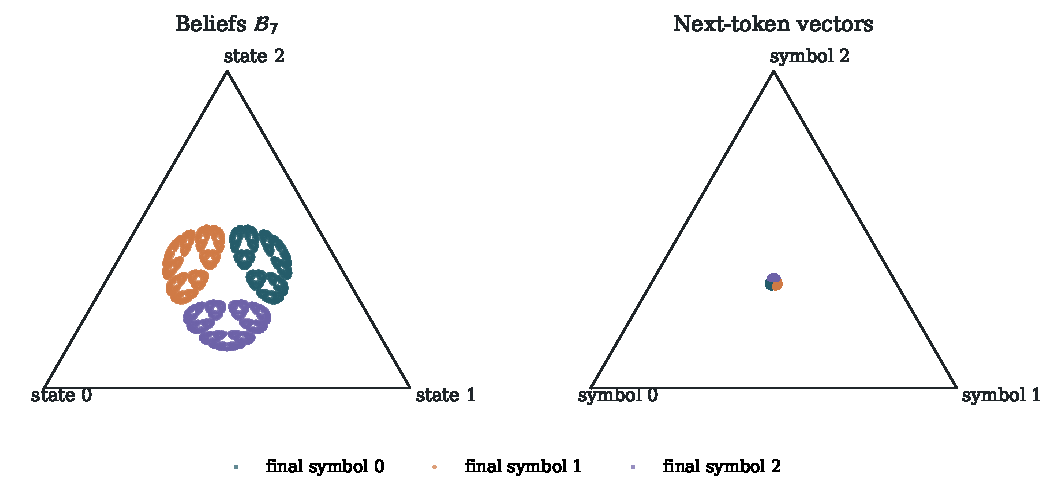
\includegraphics[width=0.86\linewidth]
                {figures/mess3-belief-and-next-token-geometry.pdf}
            \end{center}

            At a point $\eta$, the three outgoing edges are obtained by
            applying $F_0,F_1,F_2$ and have probabilities given by the three
            coordinates of $\eta A$. Thus the three geometric copies visible
            at the next depth are also the three symbol-labelled branches of
            the belief-state automaton.

          \item A belief and the observed symbol determine a unique updated
            belief $F_a(\eta)$, so the belief-state presentation is unifilar.
            The original generator is nonunifilar because its current hidden
            state and emitted symbol can leave several possible next hidden
            states. For the Simple Nonunifilar Source the reachable beliefs
            form a one-dimensional ladder, with each $1$-edge resetting to
            $\eta_0$. For Mess3 every symbol remains possible and the three
            update maps generate a rapidly branching, self-similar geometry.
            Finally, finite words form a countable set, so their image under
            the belief map is countable. Taking the closure adds limiting
            beliefs and can produce an uncountable fractal set.
        \end{subparts}
    \end{parts}
  \end{solution}
\end{exercise}
}

\begin{exercise}{Belief states and a lossy next-token readout}
  Continue with the Zero--One--Random HMM from Exercise 1, using state order
  $(0,1,R)$. For an allowable history $x_{1:n}=x_1\cdots x_n$, compute its
  belief from scratch as
  \[
    \eta^{(x_{1:n})}
      :=\frac{\eta^{(\emptyset)}T^{(x_1)}\cdots T^{(x_n)}}
        {\eta^{(\emptyset)}T^{(x_1)}\cdots T^{(x_n)}\mathbf 1}.
  \]
  Here $\eta_i^{(x_{1:n})}=\Pr(S_n=i\mid X_{1:n}=x_{1:n})$. For an allowable
  extension $x_{1:n+1}=x_{1:n}a$, update recursively as
  \[
    \eta^{(x_{1:n+1})}
      =\frac{\eta^{(x_{1:n})}T^{(a)}}
        {\eta^{(x_{1:n})}T^{(a)}\mathbf 1}.
  \]

  \begin{parts}
    \item Compute $\eta^{(0)}$ and $\eta^{(1)}$. Interpret their components
      as posterior probabilities over the three hidden phases.

    \item Show that the seven beliefs
      \[
        \mathcal B=
        \bigl\{
          \eta^{(\emptyset)},\eta^{(0)},\eta^{(1)},\eta^{(00)},
          \eta^{(01)},\eta^{(10)},\eta^{(11)}
        \bigr\}
      \]
      are distinct and that $\mathcal B$ is closed under every allowable
      symbol update. Draw the symbol-labelled transition diagram on
      $\mathcal B$.

    \item Compare your belief-state diagram with both the causal-state
      automaton constructed in Part 2 and the three-state generative HMM from
      Exercise 1.
      \begin{subparts}
        \item Match each belief to the causal state with the same
          shortest-length representative. Do the symbol-labelled transitions
          agree?

        \item Which beliefs correspond to knowing the hidden phase exactly,
          and which represent uncertainty over several phases? Show that the
          hidden phase becomes known after at most three observations and
          remains known thereafter.

        \item Observe that the finite-history belief-state presentation has
          seven states while the generative HMM has only three. What does this
          suggest about the possible relative difficulty of generation and
          inference?
      \end{subparts}

    \item For each belief $\eta^{(x_{1:n})}\in\mathcal B$ from part (b),
      compute its associated next-token probability vector
      \[
        p^{(x_{1:n})}
        :=\left(
          \Pr(X_{n+1}=a\mid X_{1:n}=x_{1:n})
        \right)_{a\in\{0,1\}}
        =\eta^{(x_{1:n})}A,
        \qquad
        A_{ia}:=\sum_jT^{(a)}_{ij}.
      \]
      Visualise the belief geometry on the $2$-simplex over hidden states
      $(0,1,R)$ and the next-token geometry on the $1$-simplex over symbols
      $(0,1)$.

    \item Calculate
      \[
        \Pr(X_{3:4}=00\mid X_{1:2}=10)
        \qquad\text{and}\qquad
        \Pr(X_{3:4}=00\mid X_{1:2}=01).
      \]
      Deduce that the next-token probability vector need not be sufficient for
      predicting the entire future.

    \item \textbf{Extension.} Let
      $\delta:=\eta^{(10)}-\eta^{(01)}$. Show that
      \[
        \delta A=0
        \qquad\text{but}\qquad
        \delta T^{(0)}T^{(0)}\mathbf 1\neq0.
      \]
      Interpret these two statements in terms of one-step and longer-horizon
      prediction.
  \end{parts}

  \begin{solution}
    \begin{parts}
      \item Multiplying the initial belief by the two symbol matrices gives
        \[
          \eta^{(\emptyset)}T^{(0)}
            =\begin{bmatrix}(1-p)/3&1/3&0\end{bmatrix},
          \qquad
          \eta^{(\emptyset)}T^{(1)}
            =\begin{bmatrix}p/3&0&1/3\end{bmatrix}.
        \]
        Their row sums are respectively $(2-p)/3$ and $(1+p)/3$.
        Normalising therefore gives
        \[
          \eta^{(0)}
            =\begin{bmatrix}\dfrac{1-p}{2-p}&\dfrac1{2-p}&0\end{bmatrix},
          \qquad
          \eta^{(1)}
            =\begin{bmatrix}\dfrac p{1+p}&0&\dfrac1{1+p}\end{bmatrix}.
        \]
        After observing $0$, the current phase is either $0$ or $1$ with the
        displayed posterior probabilities, and cannot be $R$. After observing
        $1$, it is either $0$ or $R$, and cannot be $1$.

      \item Direct evaluation gives
        \[
          \begin{aligned}
            \eta^{(00)}&=\begin{bmatrix}0&1&0\end{bmatrix},&
            \eta^{(01)}&=\begin{bmatrix}0&0&1\end{bmatrix},\\
            \eta^{(10)}&=\begin{bmatrix}1-p&p&0\end{bmatrix},&
            \eta^{(11)}&=\begin{bmatrix}1&0&0\end{bmatrix}.
          \end{aligned}
        \]
        Thus the pure beliefs are $\eta^{(11)}$, $\eta^{(00)}$, and
        $\eta^{(01)}$.
        The pure beliefs are distinct. The beliefs
        $\eta^{(\emptyset)}$, $\eta^{(0)}$, and $\eta^{(1)}$ have different
        supports from one another and from the pure beliefs. The only remaining
        comparison is between $\eta^{(0)}$ and $\eta^{(10)}$, which both have
        support $\{0,1\}$. Equality would require
        $1/(2-p)=p$, or $(1-p)^2=0$, contrary to $p<1$.

        The allowable updates are
        \[
          \begin{array}{c|cc}
            \text{current belief} & 0 & 1\\
            \hline
            \eta^{(\emptyset)} & \eta^{(0)} & \eta^{(1)}\\
            \eta^{(0)}         & \eta^{(00)} & \eta^{(01)}\\
            \eta^{(1)}         & \eta^{(10)} & \eta^{(11)}\\
            \eta^{(10)}        & \eta^{(00)} & \eta^{(01)}\\
            \eta^{(11)}        & \eta^{(00)} & \text{impossible}\\
            \eta^{(00)}        & \text{impossible} & \eta^{(01)}\\
            \eta^{(01)}        & \eta^{(11)} & \eta^{(11)}
          \end{array}
        \]
        This table specifies the requested symbol-labelled diagram and shows
        that every allowable update stays in $\mathcal B$.

      \item
        \begin{subparts}
          \item Under the assumptions used in Part 2, the correspondence is
            \[
              \begin{aligned}
                \epsilon(\emptyset)&\longleftrightarrow\eta^{(\emptyset)},&
                \epsilon(0)&\longleftrightarrow\eta^{(0)},&
                \epsilon(1)&\longleftrightarrow\eta^{(1)},\\
                \epsilon(10)&\longleftrightarrow\eta^{(10)},&
                \epsilon(11)&\longleftrightarrow\eta^{(11)},&
                \epsilon(00)&\longleftrightarrow\eta^{(00)},&
                \epsilon(01)&\longleftrightarrow\eta^{(01)}.
              \end{aligned}
            \]
            The transition table from part (b) agrees with the causal-state
            automaton after making these substitutions.

          \item The pure beliefs $\eta^{(11)}$, $\eta^{(00)}$, and
            $\eta^{(01)}$ identify the hidden phase exactly. The other four
            beliefs assign positive probability to more than one phase and
            therefore represent uncertainty.
            After two observations only the history $10$ leaves a mixed
            belief. Either allowable third symbol sends $\eta^{(10)}$ to a
            pure belief. Once the belief is pure, every allowable transition
            in the table leads to another pure belief, so the phase remains
            known.

          \item The generator has access to its actual hidden phase and needs
            only the three states $0$, $1$, and $R$. An observer begins with
            an unknown phase and must also represent four transient posterior
            distributions before synchronising with the generator. This
            example therefore shows that inference can require a richer state
            description than a particular generative presentation.
        \end{subparts}

      \item The probability of each symbol from a hidden phase is obtained by
        summing the corresponding row of its symbol matrix over destination
        states. With column order $(0,1)$, this gives
        \[
          A=
          \begin{bmatrix}
            1&0\\
            0&1\\
            1-p&p
          \end{bmatrix}.
        \]
        Hence
        \[
          \begin{array}{c|c}
            \text{belief} & \text{next-token vector}\\
            \hline
            \eta^{(\emptyset)} &
              p^{(\emptyset)}=
              \left(\dfrac{2-p}{3},\dfrac{1+p}{3}\right)\\[1mm]
            \eta^{(0)} &
              p^{(0)}=
              \left(\dfrac{1-p}{2-p},\dfrac{1}{2-p}\right)\\[1mm]
            \eta^{(1)} &
              p^{(1)}=
              \left(\dfrac{1}{1+p},\dfrac{p}{1+p}\right)\\[1mm]
            \eta^{(00)} & p^{(00)}=(0,1)\\
            \eta^{(01)} & p^{(01)}=(1-p,p)\\
            \eta^{(10)} & p^{(10)}=(1-p,p)\\
            \eta^{(11)} & p^{(11)}=(1,0)
          \end{array}
        \]
        On the belief $2$-simplex, $\eta^{(11)}$, $\eta^{(00)}$, and
        $\eta^{(01)}$ are the three vertices, while
        $\eta^{(\emptyset)}$ is the barycentre. The beliefs $\eta^{(0)}$ and
        $\eta^{(10)}$ lie on the edge joining $\eta^{(11)}$ to
        $\eta^{(00)}$, and $\eta^{(1)}$ lies on the edge joining
        $\eta^{(11)}$ to $\eta^{(01)}$.

        On the next-token $1$-simplex, each point is located by the second
        coordinate in the table, namely its probability of emitting $1$.
        The relation $p^{(x_{1:n})}=\eta^{(x_{1:n})}A$ maps the two distinct
        beliefs $\eta^{(01)}$ and $\eta^{(10)}$ to the same point
        $p^{(01)}=p^{(10)}=(1-p,p)$.

      \item Starting from $\eta^{(10)}=(1-p,p,0)$, observing a $0$ can only
        come from phase $0$ and moves the process to phase $1$, which cannot
        emit a second $0$. Hence
        \[
          \Pr(X_{3:4}=00\mid X_{1:2}=10)
            =\eta^{(10)}T^{(0)}T^{(0)}\mathbf 1=0.
        \]
        Starting from $\eta^{(01)}=(0,0,1)$, the first $0$ has probability
        $1-p$ and moves the process to phase $0$, which emits the second $0$
        deterministically. Therefore
        \[
          \Pr(X_{3:4}=00\mid X_{1:2}=01)
            =\eta^{(01)}T^{(0)}T^{(0)}\mathbf 1=1-p.
        \]
        The histories agree about the next symbol but disagree about a
        two-symbol continuation, so their shared next-token vector is not
        sufficient for the entire future.

      \item We have
        \[
          \delta
            =\begin{bmatrix}1-p&p&-1\end{bmatrix}.
        \]
        Direct multiplication gives
        \[
          \delta A=\begin{bmatrix}0&0\end{bmatrix},
          \qquad
          \delta T^{(0)}T^{(0)}\mathbf 1=-(1-p)\neq0.
        \]
        Thus the difference between the beliefs is invisible to the one-step
        readout but visible to a readout associated with the two-symbol future
        $00$.
    \end{parts}
  \end{solution}
\end{exercise}

\messThreeExercise

\begin{exercise}{Generalised hidden Markov models and predictive vectors}
  A $d$-dimensional generalised hidden Markov model (GHMM) consists of a
  finite alphabet $\mathcal X$, real $d\times d$ matrices
  $(T^{(a)})_{a\in\mathcal X}$, an initial row vector
  $\eta^{(\emptyset)}$, and a column vector $\phi$. Writing
  \[
    T:=\sum_{a\in\mathcal X}T^{(a)},
  \]
  these objects satisfy
  \[
    T\phi=\phi,\qquad
    \eta^{(\emptyset)}\phi=1,\qquad
    \eta^{(\emptyset)}T^{(x_1)}\cdots T^{(x_n)}\phi\geq0
  \]
  for every $x_{1:n}\in\mathcal X^n$ and every $n\geq0$.

  \begin{parts}
    \item \textbf{A probability law from matrix products.}
      Consider
      \[
        \Pr(X_{1:n}=x_{1:n})
          =\eta^{(\emptyset)}
            T^{(x_1)}\cdots T^{(x_n)}\phi.
      \]
      \begin{subparts}
        \item Show that these quantities are nonnegative and that
          \[
            \sum_{x_{1:n}\in\mathcal X^n}
              \Pr(X_{1:n}=x_{1:n})=1
          \]
          for every $n\geq0$.

        \item Show that
          \[
            \sum_{a\in\mathcal X}
              \Pr(X_{1:n+1}=x_{1:n}a)
              =\Pr(X_{1:n}=x_{1:n}).
          \]
          Explain why this is the consistency condition needed to define a
          one-sided stochastic process.

        \item The GHMM conditions do not require
          $\eta^{(\emptyset)}T=\eta^{(\emptyset)}$. Explain why the process
          need not therefore be stationary. Show that this additional
          equality is sufficient for stationarity.
      \end{subparts}

    \item \textbf{Predictive vectors.}
      For any $x_{1:n}$ satisfying
      $\Pr(X_{1:n}=x_{1:n})>0$, define its predictive vector by
      \[
        \eta^{(x_{1:n})}
          :=\frac{\eta^{(\emptyset)}
              T^{(x_1)}\cdots T^{(x_n)}}
            {\eta^{(\emptyset)}
              T^{(x_1)}\cdots T^{(x_n)}\phi}.
      \]
      \begin{subparts}
        \item Show that
          \[
            \eta^{(x_{1:n})}\phi=1
          \]
          and, for every continuation $y_{1:m}$,
          \[
            \Pr(X_{n+1:n+m}=y_{1:m}\mid X_{1:n}=x_{1:n})
              =\eta^{(x_{1:n})}
                T^{(y_1)}\cdots T^{(y_m)}\phi.
          \]

        \item Derive the recursive update and identify its normalising
          factor:
          \[
            \eta^{(x_{1:n}a)}
              =\frac{\eta^{(x_{1:n})}T^{(a)}}
                {\eta^{(x_{1:n})}T^{(a)}\phi},
            \qquad
            \Pr(X_{n+1}=a\mid X_{1:n}=x_{1:n})
              =\eta^{(x_{1:n})}T^{(a)}\phi.
          \]

        \item Conceptually contrast an HMM belief state with a GHMM
          predictive vector. Compare the meaning of their coordinates, their
          positivity and normalisation properties, and how they encode
          predictions of future observations.
      \end{subparts}

    \item \textbf{Predictive vectors need not be probability vectors.}
      Consider the two-state HMM
      \[
        M^{(0)}=
          \begin{bmatrix}\tfrac45&0\\0&\tfrac15\end{bmatrix},
        \qquad
        M^{(1)}=
          \begin{bmatrix}\tfrac15&0\\0&\tfrac45\end{bmatrix},
        \qquad
        \alpha=\begin{bmatrix}\tfrac12&\tfrac12\end{bmatrix}.
      \]
      Thus a hidden state is selected initially and thereafter emits a biased
      coin without changing state. Let
      \[
        S=\begin{bmatrix}2&-1\\0&1\end{bmatrix},
        \qquad
        T^{(a)}:=S^{-1}M^{(a)}S,\qquad
        \eta^{(\emptyset)}:=\alpha S,\qquad
        \phi:=S^{-1}\mathbf 1.
      \]
      \begin{subparts}
        \item Compute $T^{(0)},T^{(1)},\eta^{(\emptyset)}$, and $\phi$.
          Show that, for every $x_{1:n}$,
          \[
            \eta^{(\emptyset)}
              T^{(x_1)}\cdots T^{(x_n)}\phi
              =
            \alpha M^{(x_1)}\cdots M^{(x_n)}\mathbf 1.
          \]
          Deduce that this change of coordinates gives a valid GHMM for the
          same process.

        \item Compute $\eta^{(0)}$ and $\eta^{(1)}$. Verify directly from
          $\eta^{(0)}$ that
          \[
            \Pr(X_2=0\mid X_1=0)=\frac{17}{25},
            \qquad
            \Pr(X_2=1\mid X_1=0)=\frac8{25}.
          \]
          Explain why the entries of a GHMM predictive vector need not
          themselves be probabilities.
      \end{subparts}

    \item \textbf{The probability matrix and minimal dimension.}
      For finite sets $\mathcal U,\mathcal V\subseteq\mathcal X^*$, define
      the probability matrix by
      \[
        \mathsf P_{\mathcal U,\mathcal V}(u,v)
          :=\Pr(X_{1:|u|+|v|}=uv),
        \qquad u\in\mathcal U,\quad v\in\mathcal V.
      \]
      \begin{subparts}
        \item Use the GHMM matrix product to factor
          $\mathsf P_{\mathcal U,\mathcal V}$ as a matrix of prefix row
          vectors times a matrix of continuation column vectors. Deduce that
          \[
            \operatorname{rank}\mathsf P_{\mathcal U,\mathcal V}\leq d
          \]
          for every $d$-dimensional GHMM realisation.

        \item For the process in part (c), take
          $\mathcal U=\mathcal V=\{\emptyset,0,1\}$. Compute
          $\mathsf P_{\mathcal U,\mathcal V}$ and use an SVD to find its
          singular values. Deduce that the two-dimensional GHMM is
          minimal-dimensional.
      \end{subparts}

  \end{parts}

  \begin{solution}
    \small
    \setlist[enumerate]{itemsep=1pt,topsep=3pt,parsep=0pt,partopsep=0pt}
    \begin{parts}
      \item
        \begin{subparts}
          \item Nonnegativity is one of the GHMM assumptions. Expanding the
            product of the sum of the symbol matrices gives
            \[
              \sum_{x_{1:n}\in\mathcal X^n}
                T^{(x_1)}\cdots T^{(x_n)}=T^n.
            \]
            Hence
            \[
              \sum_{x_{1:n}\in\mathcal X^n}
                \Pr(X_{1:n}=x_{1:n})
                =\eta^{(\emptyset)}T^n\phi
                =\eta^{(\emptyset)}\phi=1,
            \]
            where $T^n\phi=\phi$ follows from $T\phi=\phi$. For $n=0$
            this also says that the empty history has probability one.

          \item Summing over the final symbol gives
            \[
              \begin{aligned}
                \sum_{a\in\mathcal X}
                  \Pr(X_{1:n+1}=x_{1:n}a)
                  &=
                  \eta^{(\emptyset)}
                    T^{(x_1)}\cdots T^{(x_n)}
                    \left(\sum_{a\in\mathcal X}T^{(a)}\right)\phi\\
                  &=
                  \eta^{(\emptyset)}
                    T^{(x_1)}\cdots T^{(x_n)}T\phi\\
                  &=\Pr(X_{1:n}=x_{1:n}).
              \end{aligned}
            \]
            Thus the length-$n$ distribution is the marginal of the
            length-$(n+1)$ distribution over its final coordinate, as
            required for a process indexed by $1,2,\ldots$.

          \item The displayed GHMM conditions relate distributions at
            successive lengths but do not say that a block has the same
            distribution after shifting its time indices. If
            $\eta^{(\emptyset)}T=\eta^{(\emptyset)}$, then
            \[
              \begin{aligned}
                \sum_{a\in\mathcal X}
                  \Pr(X_{1:n+1}=a x_{1:n})
                  &=
                  \eta^{(\emptyset)}T
                    T^{(x_1)}\cdots T^{(x_n)}\phi\\
                  &=
                  \eta^{(\emptyset)}
                    T^{(x_1)}\cdots T^{(x_n)}\phi\\
                  &=\Pr(X_{1:n}=x_{1:n}).
              \end{aligned}
            \]
            The left side is
            $\Pr(X_{2:n+1}=x_{1:n})$, so the block distributions are
            invariant under a one-step shift. Iteration gives stationarity.
        \end{subparts}

      \item
        \begin{subparts}
          \item The denominator in the definition is
            $\Pr(X_{1:n}=x_{1:n})$, and so
            \[
              \eta^{(x_{1:n})}\phi=1.
            \]
            By the definition of conditional probability,
            \[
              \begin{aligned}
                &\Pr(X_{n+1:n+m}=y_{1:m}\mid X_{1:n}=x_{1:n})\\
                &\quad=
                  \frac{\eta^{(\emptyset)}
                    T^{(x_1)}\cdots T^{(x_n)}
                    T^{(y_1)}\cdots T^{(y_m)}\phi}
                  {\eta^{(\emptyset)}
                    T^{(x_1)}\cdots T^{(x_n)}\phi}\\
                &\quad=
                  \eta^{(x_{1:n})}
                    T^{(y_1)}\cdots T^{(y_m)}\phi.
              \end{aligned}
            \]

          \item Taking $m=1$ in part (i) gives
            \[
              \Pr(X_{n+1}=a\mid X_{1:n}=x_{1:n})
                =\eta^{(x_{1:n})}T^{(a)}\phi,
              \qquad
              \eta^{(x_{1:n}a)}
                =\frac{\eta^{(x_{1:n})}T^{(a)}}
                  {\eta^{(x_{1:n})}T^{(a)}\phi}.
            \]
            The first quantity is exactly the normalising factor in the
            update shown by the second equality.

          \item An HMM belief state has coordinates
            $\Pr(S_n=i\mid X_{1:n}=x_{1:n})$, so they are nonnegative, sum to
            one, and refer to mutually exclusive hidden states. Predictive
            vectors are coordinates in a linear realisation: they need only
            satisfy $\eta^{(x_{1:n})}\phi=1$ and may have negative entries.
            Both summarise the history sufficiently to compute future-word
            probabilities through symbol-matrix products.
        \end{subparts}

      \item
        \begin{subparts}
          \item Since
            \[
              S^{-1}=
                \begin{bmatrix}\tfrac12&\tfrac12\\0&1\end{bmatrix},
            \]
            direct calculation gives
            \[
              T^{(0)}=
                \begin{bmatrix}\tfrac45&-\tfrac3{10}\\0&\tfrac15\end{bmatrix},
              \qquad
              T^{(1)}=
                \begin{bmatrix}\tfrac15&\tfrac3{10}\\0&\tfrac45\end{bmatrix},
            \]
            and
            \[
              \eta^{(\emptyset)}=\begin{bmatrix}1&0\end{bmatrix},
              \qquad
              \phi=\begin{bmatrix}1\\1\end{bmatrix}.
            \]
            In particular $T=T^{(0)}+T^{(1)}=I$, so $T\phi=\phi$, and
            $\eta^{(\emptyset)}\phi=1$. In a product, adjacent factors
            $SS^{-1}$ cancel:
            \[
              \begin{aligned}
                \eta^{(\emptyset)}
                  T^{(x_1)}\cdots T^{(x_n)}\phi
                  &=
                  \alpha S(S^{-1}M^{(x_1)}S)\cdots
                    (S^{-1}M^{(x_n)}S)S^{-1}\mathbf1\\
                  &=\alpha M^{(x_1)}\cdots M^{(x_n)}\mathbf1.
              \end{aligned}
            \]
            The right side is an HMM sequence probability and is therefore
            nonnegative. All GHMM conditions are satisfied, and both
            realisations define the same process.

          \item Both first-symbol probabilities are $1/2$. Normalising gives
            \[
              \eta^{(0)}
                =\begin{bmatrix}\tfrac85&-\tfrac35\end{bmatrix},
              \qquad
              \eta^{(1)}
                =\begin{bmatrix}\tfrac25&\tfrac35\end{bmatrix}.
            \]
            Moreover,
            \[
              T^{(0)}\phi
                =\begin{bmatrix}\tfrac12\\[1mm]\tfrac15\end{bmatrix},
              \qquad
              T^{(1)}\phi
                =\begin{bmatrix}\tfrac12\\[1mm]\tfrac45\end{bmatrix}.
            \]
            Hence
            \[
              \eta^{(0)}T^{(0)}\phi=\frac{17}{25},
              \qquad
              \eta^{(0)}T^{(1)}\phi=\frac8{25}.
            \]
            Although the second coordinate of $\eta^{(0)}$ is negative, all
            continuation probabilities obtained from it are valid. The
            predictive vector consists of coordinates in a chosen linear
            representation; unlike an HMM belief, its entries do not have to
            describe mutually exclusive hidden events.
        \end{subparts}

      \item
        \begin{subparts}
          \item For $u=u_1\cdots u_r$ and $v=v_1\cdots v_s$,
            \[
              \mathsf P_{\mathcal U,\mathcal V}(u,v)
                =
                \bigl(\eta^{(\emptyset)}
                  T^{(u_1)}\cdots T^{(u_r)}\bigr)
                \bigl(T^{(v_1)}\cdots T^{(v_s)}\phi\bigr).
            \]
            Collecting the first factors as rows and the second factors as
            columns gives the requested factorisation through
            $\mathbb R^d$. The rank of the product is therefore at most $d$.

          \item The required probabilities are
            \[
              \begin{aligned}
                \Pr(X_1=0)=\Pr(X_1=1)&=\frac12,\\
                \Pr(X_{1:2}=00)=\Pr(X_{1:2}=11)&=\frac{17}{50},&
                \Pr(X_{1:2}=01)=\Pr(X_{1:2}=10)&=\frac4{25}.
              \end{aligned}
            \]
            Thus, in the order $(\emptyset,0,1)$,
            \[
              \mathsf P_{\mathcal U,\mathcal V}
                =
                \begin{bmatrix}
                  1&\tfrac12&\tfrac12\\
                  \tfrac12&\tfrac{17}{50}&\tfrac4{25}\\
                  \tfrac12&\tfrac4{25}&\tfrac{17}{50}
                \end{bmatrix},
              \qquad
              \sigma(\mathsf P_{\mathcal U,\mathcal V})
                =\left(\frac32,\frac9{50},0\right).
            \]
            It therefore has rank two. Every GHMM realisation must have
            dimension at least two, while part (c) supplies a
            two-dimensional realisation. It is minimal-dimensional.
        \end{subparts}

    \end{parts}
  \end{solution}
\end{exercise}
